 %!TeX root = ../main.tex  
\chapter{非热化电子辐射现象的数值研究}
%\section*{引言}
ECE信号在托卡马克放电过程中总是在特定条件下出现反常升高的现象,对于这种奇怪的ECE信号很多文献只指出这是非热化电子导致,但究竟为什么会出现这种现象一直没有令人满意的解释。现在有了动理学数值研究平台,对于特殊辐射信号产生的物理过程,我们就具备了一定的分析手段。
本章主要是利用动理学数值研究平台模拟托卡马克放电参数下电子回旋辐射的变化,分析实验过程中ECEI信号变化的物理原因,包括放电前端峰的形成,密度下降过程中逃逸电子的变化等。                                                                                                                                                                                  
\section{放电前期ECE信号前端峰的形成 }\label{sec:startup}
\subsection{前端峰现象}
如\autoref{fig:dispars}(b)ECE信号所示,托卡马克放电前期ECE信号经常会出现反常升高的现象,随着密度上升这些异常升高的电子辐射又出
现下降的趋势,我们称这种ECE变化的信号为前端峰。\autoref{fig:dispars}(a)为该炮放电参数下ECEI诊断系统
在EAST装置观测区间,\autoref{fig:dispars}(b)为放电爬升期各诊断数据,从上往下分别为环电压
Vloop、电流Ip、弦平均密度$n_e$、硬X射线HX、软X射线SX以及电子回旋辐射ECE。该放电特征在低密度放电前期中具有相当的普遍性,因此我们以此炮放电参数为分析对象,研
究在该背景参数下非热化电子的分布演化以及对应的电子回旋辐射变化,尝试解释前端峰出现的物理
过程。我们的研究思路是这样的:通过将诊断测量的宏观背景参数连续输入动理学模型驱动分布函数
演化,以此研究电子回旋辐射信号的变化过程,进而和实验中ECE信号对比并给出不同阶段辐射强度
变化的物理原因。模拟过程中需要的背景宏观参数由实验测得,有电子密度、环电压等。
\begin{figure}
\centering
\includegraphics[width=14cm]{image96_2.png}
\caption{\label{fig:dispars}(a)ECEI观测区域示意图 (b)EAST放电参数图}
\end{figure}
\subsection{模拟参数设置}
我们以托卡马克芯部诊断数据为背景参数,模拟时间区间为0.3~s-0.8~s。假设在该时间段等离子体已经具备了一定的温度,由于放电初期等离子体芯部电子温度没有有效的诊断手段,这里就取 $T_e$=0.5~KeV、0.7~KeV、0.9~KeV三种温度作为参考组,取平均环电压E=-0.077~V/m,密度由极化干涉仪提供,为时变输入参数(\autoref{fig:Expne-ece}所示),磁场强度$B_0=2.46~T$,有效电荷数Z=1,磁扰动为0,以上为程序计算所依赖的输入参数。

为了计算电子回旋辐射强度,我们假设逃逸电子主要处于|r|<a/2区域,在该区间温度、磁场和密度满足空间均匀分布,该区域的分布函数由动理学给出。|r|>a/2区域分布函数满足热分布,具有特定的温度分布剖面。\autoref{fig:simparset}为0.7s时磁场、温度和密度沿小半径的分布,中间平坦区间的分布函数由动理学给出,温度和密度在|r|>a/2区间满足二次函数分布,速度分布函数满足麦克斯韦分布。虽然磁场实际分布并不是如此,这样做主要是为了设置均匀背景环境,使分布函数与空间无关,减少计算量,同时磁场导致的回旋辐射阻尼主要体现在几十MeV高能逃逸电子,对百KeV非热化电子影响可以忽略不计,而电子回旋辐射一般主要来源于百KeV非热化电子,因此原则上不会影响最终计算结果。用于模拟的电子回旋频率113.5~GHz对应托卡马克中2次冷等离子体回旋频率位置r=0.4~m。由于放电前期密度小于$5×10^{18}~m^{-3}$温度小于0.5~KeV,根据Bornatic公式\cite{RN351},对应的2X模光学厚度均小于1,满足光学薄条件,此时电子回旋辐射主要来自于观测点内部的非热化电子辐射。


在计算网格参数设置方面,这里取约化动量范围为p=[0,9],该区间设置了270个格点,勒让德数nL=55,约化时间步长$dτ=2×10^{-3}$,约化因子为电子相对论碰撞频率$ν_{cc}=\frac{e^4 nlnΛ}{4πϵ_0^2 m_e^2 c^3 }$。完成分布演化计算后,电子回旋辐射程序根据每个时刻的分布函数求解各径向位置发射率和吸收系数,最后通过路径积分获得辐射强度。\autoref{fig:Sim-ece}为113.5~GHz电子回旋辐射在三种不同芯部电子温度下的辐射强度时序图。由\autoref{fig:Sim-ece}可以看出,背景温度越高对应的辐射强度越大,但是具有相似的辐射形状,由于放电初期等离子体刚刚建立,一般温度不会超过0.5~KeV,这里选取$T_B=0.5~KeV$具体分析电子回旋辐射演化过程中分布函数的变化。
\begin{figure}[H]
\centering
\includegraphics[width=12cm]{image96.png}
\caption{\label{fig:simparset}用于计算电子回旋辐射的背景参数分布,从上往下分别表示纵场、温度、密度分布,橘红色区间表示113.5~GhZ冷等离子体共振层位置}
\end{figure}

\begin{figure}[H]
\centering
\includegraphics[width=12cm]{image97.png}
\caption{\label{fig:Expne-ece}EAST \#64987频率为113~Ghz电子回旋辐射和等离子体密度时序图,$t_c$表示密度突然上升时间}
\end{figure}

\begin{figure}
\centering
\includegraphics[width=12cm]{image98.png}
\caption{\label{fig:Sim-ece} 三种不同背景温度下频率为113.5Ghz电子回旋辐射时序图}
\end{figure}
\subsection{实验现象的数值分析}
如\autoref{fig:Sim-ece}所示,模拟结果中芯部温度为0.5~keV的电子回旋辐射信号和实际辐射信号\autoref{fig:Expne-ece}在宏观上均出现了类似前端峰的结构,虽然在细节上有不同的地方。例如\autoref{fig:Sim-ece}模拟中辐射信号迅速上升然后在0.35~s时间附近达到前端峰平台区间,而实际电子回旋辐射信号\autoref{fig:Expne-ece}在0.3~s之前几乎没有明显信号,直到 0.3~s后才开始缓慢爬升并于0.45~s达到前端峰平台。放电初期等离子体背景参数复杂性导致这种差异的原因有很多:首先是等离子体温度的变化,姑且假设0.3~s后等离子体具有热分布特征,模拟中取固定的电子温度实际上无法反映真实的温度变化过程。如果考虑变化的温度,由于逃逸电子的Dreicer 电场(\autoref{eq:Dreicer_Field})与温度成反比,当放电初期等离子体温度低于0.5~keV或还不能用温度描述时,此时逃逸电子的临界电场相对较高,对应的非热化电子辐射自然就弱,随着温度逐渐升高,逃逸电子增长率上升,非热化电子辐射也逐渐升高(如\autoref{fig:Sim-ece}所示,随着背景温度上升,辐射强度也随之上升)这很有可能是实验中非热辐射缓慢上升的其中一个原因。另一个原因是托卡马克中复杂的磁场位形导致逃逸电子在静电场加速运动过程中出现无碰撞散射,使逃逸电子垂直方向回旋动能也逐渐增加\cite{RN1794} ,这也会导致电子回旋辐射强度上升。即使如此,模拟结果并不影响我们定性分析放电前期非热化电子的演化以及回旋辐射,我们主要分析以下两个阶段:前端峰爬升段和中后段。
\par \noindent
1.前端峰爬升段


如\autoref{fig:peakece1}所示,初始为热分布的等离子体在电场驱动下逐渐偏离热分布,电子回旋辐射强度也逐渐上升并在经过约0.04~s后辐射强度达到饱和,非热分布达到相对稳定的状态,从时间上看这和实验中观察到辐射上升时间0.45~s偏离较大,因此实验中辐射强度爬升的过程和模拟中看到的物理图像并不相同,而是其它物理机制导致的结果,或温度上升或电子在非均匀磁场中无碰撞散射过程\cite{RN1794}	等,具体原因还有待进一步研究。模拟中当时间达到0.34~s后非热化电子辐射强度开始出现下降的趋势,这是因为密度上升约化电场绝对强度持续下降导致非热电子成分减少。

\begin{figure}
\centering
\includegraphics[width=12cm]{image99.jpeg}
\caption{\label{fig:peakece1} 回旋辐射爬升段对应的速度分布演化过程,其中速度分布取$log_{10}⁡f$,白色半圆为托卡马克磁轴处113.5~GHz回旋辐射共振速度曲线}
\end{figure}

%\begin{figure}
%\centering
%\includegraphics[width=12cm]{image100.png}
%\caption{\label{fig:Ec-ECE} 约化电场强度E/Ec以及模拟给出的辐射温度变化曲线图}
%\end{figure}

\par \noindent
2.前端峰中后段\par
\autoref{fig:peakece2}展示了模拟给出的前端峰中后期非热化电子辐射以及速度分布的演化。在时间段1-2之间,辐射上升的原因是密度增加所导致的结果。由于113.5~Ghz辐射对应的光学厚度约为0.07远小于1,电子密度变化对辐射的影响也尤为显著,即使密度上升使得非热化电子权重减少,但数量优势还是导致了辐射强度稍稍上升;在2-4时间段出现了辐射快速上升的现象,其中原因除了密度快速上升的结果,另一个机制就是雪崩效应。由于等离子体密度迅速上升,逃逸电子和背景电子的碰撞概率增大导致短时间内大量的逃逸电子通过碰撞转化具有较高垂直速度的非热化电子。如\autoref{fig:peakece3}(a)为共振曲线上电子运动方向与辐射的权重的关系,其中$ξ=p_∥/p$,表明电子回旋辐射主要依赖于垂直方向速度,而平行方向的速度对辐射几乎没有贡献。\autoref{fig:peakece3}(b)展示了2-4时间段共振曲线上电子散射角方向分布随时间的演化过程:雪崩效应导致垂直方向速度分布逐渐增大,而约化电场下降导致平行方向速度分布逐渐减小;4-6区间,由于约化电场持续下降,逃逸电子减少,回旋辐射持续变弱。实验\autoref{fig:Expne-ece}中观测到在$t_c=0.5~s$密度迅速上升时ECE辐射出现的小峰结构,然后紧接着辐射强度下降,该过程正好对应模拟\autoref{fig:peakece2}中2-6时间出现的辐射变化。这是通过模拟首次重现了电子回旋辐射的前端峰现象。
\begin{figure}
\centering
\includegraphics[width=12cm]{image101.jpeg}
\caption{\label{fig:peakece2}电子回旋辐射小峰不同时刻对应的速度分布演化,其中颜色表示速度分布取$log_{10}f$,$T_{rad}$表示模拟得到的辐射温度}
\end{figure}


\begin{figure}[ht]
 \centering
\begin{overpic}[width=12cm]{image102.png}
 \put(83, 65){\large\bfseries\color{black}{$(a)$}}
\end{overpic}
\begin{overpic}[width=12cm]{image103.png}
 \put(83, 65){\large\bfseries\color{black}{$(b)$}}
\end{overpic}
\caption{\label{fig:peakece3}(a)共振曲线上辐射权重分布,其中$ξ=p_∥/p$;(b)共振曲线上电子速度散射角分布演化}
\end{figure}

\subsection{	雪崩效应与前端峰}
为了演示雪崩效应在前端峰的作用,我们通过程序控制雪崩算符实现无雪崩和有雪崩下非热化电子的辐射演化。\autoref{fig:peakece4}展示了雪崩效应在前端峰形成过程中的重要性:当不考虑雪崩效应时非热化电子辐射对约化电场变化非常敏感,此时非热化电子只能通过初级逃逸电子形成,当时间大于0.34~s时由于密度上升约化电场降低,初级逃逸电子辐射已经开始下降并且在0.5~s附近辐射消失;考虑雪崩碰撞后在时间大于0.34~s后高能的逃逸电子依旧有机会通过碰撞将背景电子转化为逃逸电子,迟滞了非热化电子的减少,因此才能在较长的时间保持非热辐射,这也是雪崩电子的迟滞特征\cite{RN1805}。与实验中前端峰的时间相比,只有考虑雪崩效应才能解释前端峰的时间尺度,因此前端峰的形成雪崩效应起到了重要作用。

\begin{figure}
\centering
\includegraphics[width=12cm]{image104.png}
\caption{\label{fig:peakece4}有雪崩效应和没有雪崩效应113.5~GHz电子回旋辐射以及虚线0.55~s时刻动量分布对比图}
\end{figure}

\section{密度下降过程中的回旋辐射}\label{sec:exp_ece}

EAST装置在53852炮中做了这样的实验:实验人员通过在放电平台期主动控制密度下降以研究逃逸电子的临界电场问题,放电平台期间相对于放电爬升期可以实现更好的控制变量。在放电平台期间,等离子体芯部温度始终保持在0.8-1~keV,磁轴处环向场$B_t=1.73~T$,EAST装置大半经R=1.8~m,小半径a=0.4~m。实验结果如\autoref{fig:linearne}所示,该放电为欧姆放电,不存在除欧姆场外任何加热手段。电子密度通过控制实现从$1.0-0.3×10^{19} ~m^{-3}$线性下降,等离子体电流约为0.2~MA,环电场对Connor电场$E_c$的比值从15线性增加至20。在此过程中Dreicer电场$E_D/E$约为510,$E_D$远大于背景电场,因此不会改变主体电子分布,只有少量电子发生逃逸。CdTe闪烁探测系统探测高能逃逸电子产生的HX(硬X射线),ECE系统探测能量低于100~keV的非热化电子回旋辐射。根据ECE信号和HX信号可以看出密度下降过程辐射变化主要分为两个阶段:第一阶段发生在[5-7.75]~s,ECE信号增长缓慢,几乎看不出变化,但是HX信号强度存在明显上升的趋势;第二阶段发生在7.75~s之后,此时ECE信号指数增加,HX信号反而开始下降,同时我们还可以看到等离子体电流上升以及环电压下降的趋势。
\subsection{基于双阈值电场对实现现象的解释}\label{sec:no_growth}
Zhu.X2020年于NF发表的论文\cite{RN960}对这种现象解释是逃逸电子双阈值电场的物理表现。第5~s时对应的电场$E_{th1}≈16.2×E_c$称为第一阈值电场,通过\autoref{fig:linearne}(d)可以看出在5~s后HX射线的辐射强度均开始随时间增加,说明逃逸电子的数量和能量随时间逐渐变多。论文验证了理论上初级逃逸逃逸电子增长率和实验测量的增长率在量级上比较吻合,说明这个过程中的以初级逃逸电子为主。随着密度继续下降,电子碰撞阻力持续减小,在7.75~s时达到了第二阈值电场$E_{th2}≈19.8×E_c$,此时对应的逃逸主要为雪崩逃逸为主,$E_{th2}$称为雪崩阈值电场。雪崩发生时逃逸电子通过和主体电子发生大角度碰撞导致高能的逃逸电子损失部分能量传递给被碰撞的主体电子,当碰撞出来的主体电子速度高于逃逸速度时就会转变为逃逸电子,新产生的逃逸电子和原先的逃逸电子又继续和主体电子碰撞,以此循环逃逸电子数量将会指数增长,因此称为雪崩效应。文中给出这样的结论有3点原因:1.当电场大于$E_{th2}$时环电压迅速下降、等离子体电流上升同时回旋辐射信号迅速上升(电子回旋辐射诊断主要对低于100~keV以下的大角度非热化电子敏感),说明大量低能逃逸电子产生,符合雪崩效应的产生机制;2.如\autoref{fig:linearne2}(b),通过对HX能谱分析发现电场强度大于$E_{th2}$时逃逸电子能量开始向低能转移,这与大角度碰撞的雪崩过程也相吻合;3.雪崩逃逸增长率理论公式预测的数值与HX信号损失速率接近,HX信号损失是因为逃逸电子通过碰撞传递给新的逃逸电子导致自身能量下降。

\begin{figure}
\centering
\includegraphics[width=12cm]{image105.png}
\caption{\label{fig:linearne}EAST\#53852炮放电参数图,分别为(a)约化电场Eloop/Ec,等离子体电流,(b)环电压、等离子体密度,(c)112~Ghz和121Ghz电子回旋辐射,(d)硬X射线,CdTe探测器
}
\end{figure}


\begin{figure}
\centering
\includegraphics[width=12cm]{image106.png}
\caption{\label{fig:linearne2}(a)主体等离子体内部和外部逃逸电子能量分布(b)主体等离子体内部逃逸电子在’雪崩’发生前和发生后能谱分布。能量谱分布是通过探测等离子体和scrape-off-layer区域极向阵列探测CdTe HXR探测器测得,图片来自[X. Zhu,NF,2020]\cite{RN960}}
\end{figure}


Zhu.X提出双阈值电场的理论依据是Aleynikov 2015年发表在PRL上关于双逃逸阈值电场存在性的理论分析\cite{RN1805}。该论文考虑了存在均匀磁场和电场下电子速度分布动理学过程,首先初级逃逸电子产生要求电场强度必须要大于最小运动阻尼力,该阻尼力由辐射阻尼和碰撞阻尼共同构成,克服该阻尼所需要的最小电场称为第一临界电场。由于磁场会通过回旋辐射阻尼使得逃逸电子存在能量上限,当最高能量的逃逸电子和主体电子发生大角度碰撞后,碰撞后的逃逸电子能量和被碰撞的主体电子均小于临界速度时,碰撞前的逃逸电子就会退化为主体电子,此时就不会产生雪崩逃逸。只有当碰撞后逃逸电子和主体电子均超过临界速度时才能发生雪崩逃逸。为了计算雪崩逃逸增长率,Aleynikov假设逃逸电子分布为$δ(p-p_{max} )$分布,其中$p_{max}$为逃逸电子最大动量,在对动理学方程取近似解后得到了雪崩逃逸的临界电场。然而3年后O.Embreus\cite{RN1811}		通过Boltzmann碰撞项严格数值求解雪崩过程后发现Aleynikov计算中所使用的等离子体参数并不存雪崩阈值电场。如\autoref{fig:linearne3}展示了三种模型计算逃逸电子增长率,其中Rosenbluth-Putvinski\cite{RN1793}模型未考虑回旋辐射阻尼,逃逸电子能量趋向于无穷大,自然不可能存在雪崩阈值。另一个为A\&B model即Aleynikov-Breizman模型,最后一个就是Boltzmann碰撞模型。玻尔兹曼碰撞模型计算结果永远都具有正的增长率而A\&B模型在$E<1.7E_c$逃逸电子增长率为负。造成这种区别的原因是A\&B model 对逃逸电子采用的δ分布函数,实际上逃逸电子的能量分布远大于δ函数分布,总是有足够多的逃逸电子满足雪崩效应所需能量来碰撞出新的逃逸电子。O.Embreus计算了密度$n_e=10\times10^{19}~ m^{-3}$,温度$T_e=1~keV$,有效电荷数$Z_{eff}=5$,B=1.81~T的等离子体环境并证明其不存在雪崩阈值。对于当下实验条件,密度、有效电荷数和磁场都低于O.Embreus所计算的等离子体条件,逃逸电子更容易产生,因此更加不可能出现雪崩阈值电场。


\begin{figure}
\centering
\includegraphics[width=12cm]{image107.png}
\caption{\label{fig:linearne3}三种模型下雪崩逃逸电子增长率。等离子体参数:热电子密度$n_e=10^{20} ~m^{-3}$;温度$T_e=1~KeV$;有效电荷数$Z_{eff}=5$,B=1.81~T,图片参数来自\cite{RN1811}}
\end{figure}
\subsection{磁扰动机制猜想}
综上所述,我们有理由怀疑是别的物理机制导致以上观测到的现象。 影响逃逸电子产生的除了有电场、密度等还有等离子体温度(Dreicer电场)、等离子体中波和逃逸电子的相互作用\cite{RN1815}、以及磁场扰动导致的逃逸电子损失\cite{RN1485}。由于放电平台期间密度下降过程中等离子体温度始终保持在1~keV,因此首先排除是温度的影响。等离子体波和逃逸电子共振作用会导致逃逸电子动量散射从而导致回旋辐射增加,波与逃逸电子的相互作用时间通常在毫秒量级且具有爆发性尖刺结构或台阶结构\cite{RN2102,RN1868,RN975},因此波导致回旋辐射在秒量级升高的现象可能性较小。最终我们猜测是随机磁扰动随时间的变化引起具有类似双阈值电场的实验现象。如\autoref{fig:Becene}所示,随着密度下降,在7.7~s附近高频磁探针信号涨落突然下降,同时ECE辐射信号迅速上升。根据磁信号的时频图,高频磁探针信号的频谱主要集中在400~Khz以上,说明该磁扰动主要由等离子体中随机磁扰动造成\cite{RN1485},排除磁流体力学波的可能性。为了更直观比较磁扰动和ECE信号的关系,我们对高频磁探针信号每2500个数据点取一次标准差得到\autoref{fig:Bstd},从中可以看出当磁扰动下降时ECE辐射迅速上升,因此磁扰动必然和ECE辐射有密切关系。另外从\autoref{fig:linearne2}(a)图可以看出,7.7~s等离子体外HX辐射相对8.3~s较高,说明磁扰动下降后逃逸电子约束变好,因此才导致等离子体为HX辐射下降。

\begin{figure}[ht]
\centering
\includegraphics[width=10cm]{image108.png}
\caption{\label{fig:Becene}EAST\#SHOT53852放电参数图(a)电子密度(b)121~GHz电子回旋辐射信号(c)高频磁探针信号(d)磁信号时频图}
\end{figure}

\begin{figure}[ht]
\centering
\includegraphics[width=12cm]{image109.png}
\caption{\label{fig:Bstd}高频mirnov线圈测得的磁扰动标准差与ECE信号时序图}
\end{figure}


\subsection{	模拟参数设置}

为了验证这种猜想,我们将该炮放电参数代入动理学程序中研究非热辐射和逃逸电子的变化规律。程序的输入参数如\autoref{fig:linearne5}所示,其中磁扰动正比于磁探针信号标准差,根据之前实验和理论论文\cite{RN2086,RN1485},托卡马克磁扰动δB/B约为$10^{-4}\sim10^{-5}$,所以我们也取δB/B为此量级。另外磁场B=1.73~T,温度T=1~keV。模拟中取pMax=9,动量空间格点数nP=680,勒让德数nL=55,约化时间步长$dτ=2\times10^{-2}$,模拟ece频率为87~Ghz,对应二次回旋冷等离子体共振位置约小半径0.2~m处。
\begin{figure}[ht]
\centering
\includegraphics[width=12cm]{image110.png}
\caption{\label{fig:linearne5}用于动理学模拟的输入参数时序图}
\end{figure}

\subsection{实验现象的数值分析}
通过诊断数据驱动动理学程序,我们得到了模拟和实验中ECE信号对比图。如\autoref{fig:linearne6}(a)所示,其中信号取相对变化量的log值,$ΔT=T-T_{min}$,从图中可以看出实验和模拟结果在定性上相当一致。我们还计算了逃逸电子占总体电子数量的比值,如\autoref{fig:linearne6}(b)所示。模拟给出的$n_r/n$和实验HXR之间具有很好的线性关系。为了探究密度下降过程中更多的细节,我们画出了辐射上升时间段6个时刻速度分布,如\autoref{fig:linearne7}所示,当辐射上升时电子速度分布也迅速向高能区间扩散,此时7.8~s正对应磁扰动下降。

\begin{figure}
\centering
\includegraphics[width=14cm]{image111.png}
\caption{\label{fig:linearne6}(a)实验和模拟中ECE信号相对涨落量(b) 模拟得到的逃逸电子占比和实验中硬X射线辐射强度对比图}
\end{figure}

\begin{figure}
\centering
\includegraphics[width=12cm]{image112.png}
\caption{\label{fig:linearne7}电子回旋辐射模拟时序图以及其间6个时刻速度分布图}
\end{figure}

\begin{figure}
\centering
\includegraphics[width=10cm]{image113.png}
\caption{\label{fig:linearne8}不考虑磁扰动时模拟辐射和实验辐射对比}
\end{figure}

当我们将磁扰动设置为零,辐射如\autoref{fig:linearne8}所示,很显然这与实验结果不符。
因此我们对实验中观察到的物理现象是这样理解的:在[5~s-7.7~s]内随着密度下降,约化电场强度逐渐升高,电子更容易逃逸,因此HX射线强度也逐渐上升,正如\autoref{fig:linearne6}(a),但是由于磁扰动强度较高,根据Harvey磁扰动粒子损失系数模型\cite{RN2076} (关于该方程的细节可参考\autoref{eq:Harvey})
\begin{equation}
\frac{\partial f}{\partial \tau}=-\frac{v_{\delta B}}{v_{c c}} f
\end{equation}
该方程中电子的扩散系数与动量分布有关。如\autoref{fig:linearne9}所示,电子在约化动量空间p=[0.1,1]具有较高的损失系数,高动量区间损失系数下降,这意味着能量处在[2~keV 200~keV]的电子很容易受磁扰动损失,而能量更高的逃逸电子拥有更高的约束。非热化电子的ECE信号主要由动量为0.6~mc的电子回旋辐射贡献,如\autoref{fig:linearne7}中白色半圆所示,逃逸电子在电场驱动下加速过程中,首先要穿越[0.1 ,1]区间。在7.7~s之前的时间,由于磁扰动较高,电子在 [0.1, 1]约化动量区间损失较大因此ECE信号很弱。当时间大于7.7s时磁扰动突然下降至原先的一半,逃逸电子损失减小,ECE辐射迅速上升。逃逸电子增多同时为雪崩效应提供了雪崩种子电子,在初级电子和雪崩电子的共同作用下,逃逸电流增加(\autoref{fig:linearne}(a),Ip),逃逸电流的磁屏蔽效应又导致了环电压下降(\autoref{fig:linearne}(b),Uloop)。因此所有现象的源头很有可能是磁扰动造成的,而关于ZHU.X提出的临界电场$E_{th1}$实际上取决于HXR诊断的对HX射线的能量响应,直接定义为逃逸电子的阈值电场似乎并不合适。雪崩效应实际一直都存在,只是在磁扰动降低时有了更多的逃逸电子种子,雪崩效应才更加明显。
\begin{figure}
\centering
\includegraphics[width=10cm]{image114.png}
\caption{\label{fig:linearne9}逃逸电子磁扰动损失系数与约化动量关系,其中动量方向$ξ=1(ξ=p_∥/p)$}
\end{figure}
\clearpage
\subsection{验证磁扰动猜想的另一个实验证据}
\begin{figure}[t]
\centering
\includegraphics[width=12cm]{image115.pdf}
\caption{\label{fig:linearne10}(a)EAST\#53854等离子体电流与约化环电场时序图(b)等离子体环电压与密度时序图}
\end{figure}
\begin{figure}
\centering
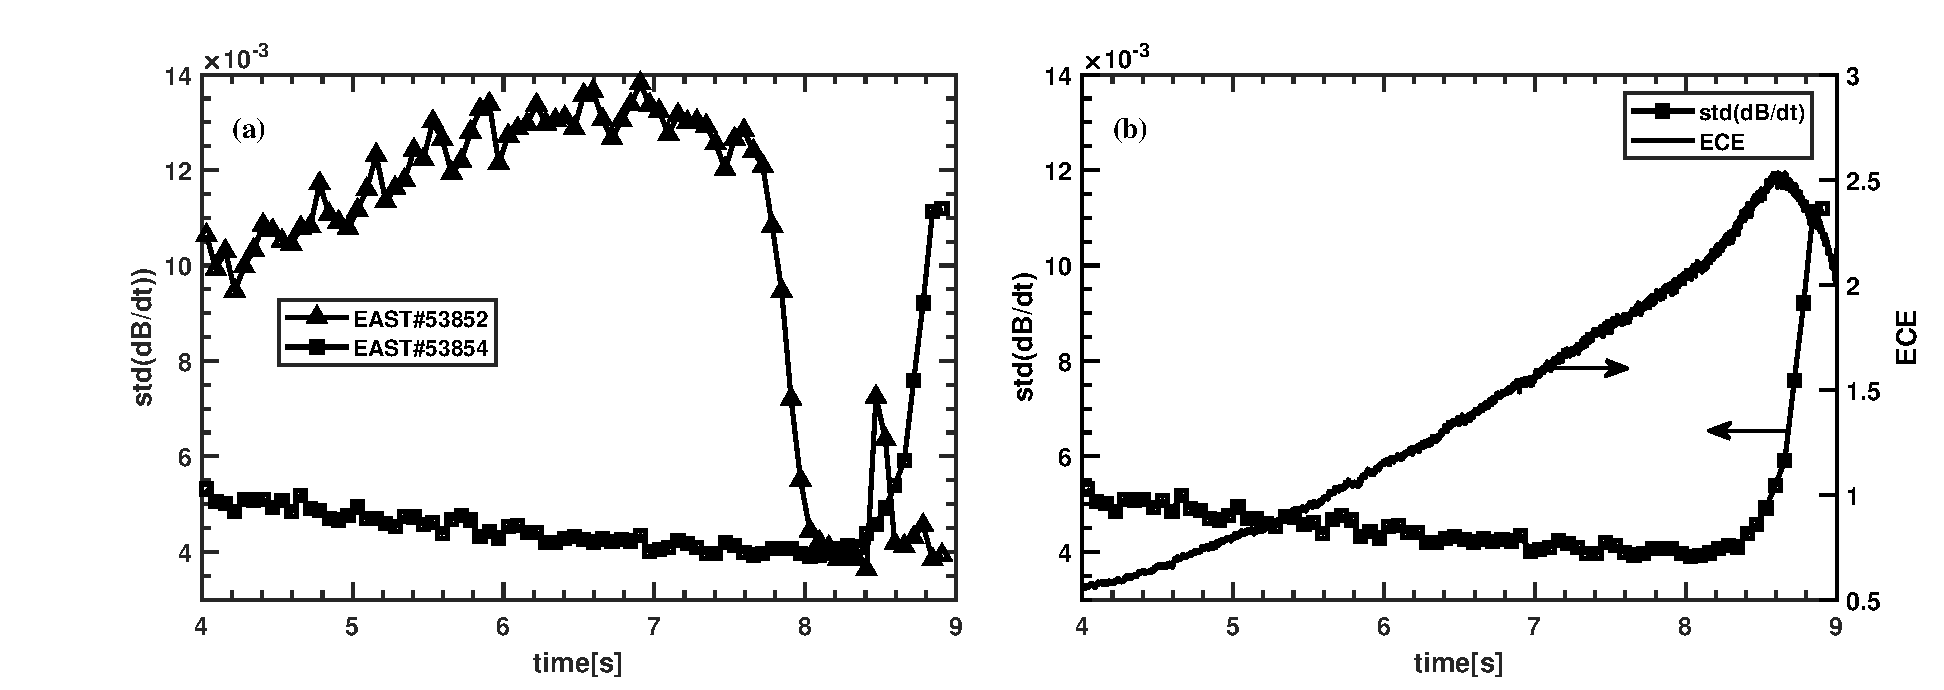
\includegraphics[width=14cm]{image116.eps}
\caption{\label{fig:linearne11}(a)EAST\#53852与EAST\#53854相同磁探针测得的磁扰动对比(b)EAST\#53854磁扰动标准差与ECE辐射}
\end{figure}
紧跟着EAST\#53852炮后的EAST\#53854可以证明以上猜想,同样是放电平台期密度下降实验,其放电参数如\autoref{fig:linearne10}所示。通过相同的低频磁探针信号(如\autoref{fig:linearne11}(a),这一炮高频磁探针信号无法使用)可以看出53854炮的磁扰动明显小于53852炮,由于逃逸电子损失小,随着约化电场增加,ECE信号也逐渐变强(\autoref{fig:linearne11}(b)),等离子体电流增大(\autoref{fig:linearne10}(a)),此时逃逸电流也相应增加,磁屏蔽效应增大,导致环电压下降(\autoref{fig:linearne10}(b))。当时间达到8.5~s时,磁扰动突然增加(如\autoref{fig:linearne11}(b)),同时ECE信号下降,等离子体电流下降,环电压增加,对应逃逸电子损失,逃逸电流下降,磁屏蔽效应下降,环电压上升,非热化电子减小,ECE辐射变弱。值得注意的是EAST\#53854炮ECE信号\autoref{fig:linearne11}(b)在[5-8]~s磁扰动很小时与无磁扰动模拟密度下降过程电子回旋辐射\autoref{fig:linearne8}很相似。因此在密度下降过程中磁扰动是导致ECE辐射变化的重要因素。  


\section{小结}
本章首次通过模拟解释了放电初期前端峰的形成过程和放电平台期密度下降过程ECE信号的变化。关于放电初期前端峰的形成,我们发现了放电初期雪崩效应是逃逸电子形成和维持过程的重要机制,因为雪崩效应的迟滞性使得逃逸电子不会因电场减小而迅速消失,使得前端峰特征时间达到了秒量级。另一方面,我们对逃逸电子观察到的双阈值电场现象提出了新的物理猜想,解释了密度下降过程ECE辐射迅速升高的原因是由于磁扰动造成。通过对这些现象的数值模拟使我们对辐射背后的物理过程有了更加深刻的认识。


